\documentclass[a4paper, twoside]{article}
\usepackage{listings}			% Used to include VHDL-code and fragments
\usepackage[english]{babel}		% English hyphenation patterns and english names 
\usepackage{pslatex}			% Times, helvetica and courier
\usepackage[T1]{fontenc}		% Nicer font-encoding
\usepackage[hidelinks]{hyperref}% Gives clickable references in pdf-file
\usepackage{graphicx}			% Used to include .pdf, .jpg and .png-files
\usepackage{tabularx}			% Used for evenly spread tables
\usepackage{eso-pic}			% Absolute positioning, used for lines-to-track appendix and front- and backpage
\usepackage{datetime}			% Used for some data-references
\usepackage[font=small,format=plain,labelfont=bf,up,textfont=up]{caption}	% Nicer captions
\usepackage{nonfloat}			% Captions for non-floating figures and tables
\usepackage{nextpage}			% Advanced nextpage commands
\usepackage{keystroke}			% "real" keys
%\usepackage[nottoc]{tocbibind}		% Include Bibliography in ToC
\usepackage{multirow}			% Span text over multiple rows
\usepackage{verbatim}			% For comment-environment
\usepackage[left=3.5cm, right=2.5cm]{geometry}
\usepackage[section]{placeins}  %zorgt ervoor dat floats niet onder een andere section komen, want dat is vervelend!
\usepackage{lmodern}
\usepackage{amsmath}
\usepackage{ntheorem}
\usepackage{a4wide}
\usepackage{cite}
\usepackage{amsfonts}
\usepackage{longtable}
\usepackage{placeins} %use \FloatBarrier to prevent figs/tabulars into other (sub)section
\usepackage{cleveref}  % the Smart Reference, just use \cref{name}.
\usepackage{csquotes} %use \enquote{text} for quotes

%%%%%%%%%%%%%%%%%%%%%%%%%%%%%%%%%%%%%%%%%%%%%%%%%%%%%%%%%%%%%%%%%%%%%%
% Settings
%%%%%%%%%%%%%%%%%%%%%%%%%%%%%%%%%%%%%%%%%%%%%%%%%%%%%%%%%%%%%%%%%%%%%%

% Settings for hyperref-package
\hypersetup{	colorlinks	= false,		%
		pdfborder	= 0 0 0}		%

% Settings for listings-package
\lstset{	numbers		= left,			%
		numberstyle	= \tiny,		%
		numbersep	= 5pt,			%
		language	= JAVA,			%
		breaklines	= true,			%
		showspaces	= false,		%
		showstringspaces= false}

%%%%%%%%%%%%%%%%%%%%%%%%%%%%%%%%%%%%%%%%%%%%%%%%%%%%%%%%%%%%%%%%%%%%%%



\begin{document}
	\newcounter{tempcounter}	% For temporarily breaking enumerate-environments

	\pagestyle{empty}		% To prevent pagenumber on backside of titlepage
	% Frontpage with image
\AddToShipoutPicture*{
	\setlength{\unitlength}{1cm}
	\put( 0,  0){
\includegraphics{images/TUDelft_border}}	%PDF version 1.5 preferred
	\put( 1, 13){\color{cyan}\linethickness{2cm}\line(0,1){7}}
	\put( 1, 13.5){\rotatebox{90}{\color{white}\large\textsf{Delft University of Technology}}}
	\put( 2, 23){\color{black}\linethickness{6cm}\line(1,0){15.5}}
	\put( 3, 25){\color{white}{\large{TI2736-A}}}
	\put( 3, 24){\color{white}{\Huge{Report Assignment 1}}}
	\put( 3, 23){\color{white}{\LARGE{Artificial Neural Network}}}
%	\put( 3, 21){\color{white}{\Huge{test}}}
%	\put( 4, 8){\includegraphics[width=11cm]{images/Matlab_graph4}}
	\put( 3,  9.5){\large{Group 19}}
	\put( 3,  9){\large{Rick Molenaar, 4280814}}
	\put( 3, 8.5){\large{Matthijs Klaassen, 4273796}}
	\put( 3,  8.0){\large{Dani\"{e}l Brouwer, 4288297}}
	\put( 3,  5){\large{\today}}
	\put( 3,  4.5){\large{Version 1.0}}
}
~
\clearpage

%	\input{versieoverzicht}
%	\input {abstract} 
    
	\pagestyle{headings}


	\clearpage
\tableofcontents
	\clearpage
    
    
%%%%%%%%%%%%%%%%%%%%%%%%%%%%%%%%%%%%%%%%%%%%%%%%%%%%%%%%%%%%%%%%%%%%%%
% 				The Input Files for each Section here:
%%%%%%%%%%%%%%%%%%%%%%%%%%%%%%%%%%%%%%%%%%%%%%%%%%%%%%%%%%%%%%%%%%%%%%
	%EXAMPLE:
	\section{Introduction} \label {chapter:introduction}

\subsection{test}
bla bla bla
           \clearpage 	
           
\section{Architecture} 
\label {chapter:architecture}
\begin{itemize}
\item 1. How many input neurons are needed for this assignment?\\\\
Ten, as there are ten initial inputs (features). The network should classify 10 features into 7 classes.
\item 2. How many output neurons do you require?\\
As was described above the network goes from 10 features (inputs) to 7 classes (outputs), so there are 7 output neurons.
\item 3. How many hidden neurons will your network have?\\
The amount of hidden neurons is not fixed. It depends on a lot of different factors and it is almost impossible to tell the optimum amount. We started testing with 10 hidden neurons per layer, but eventually settled on 50 neurons per layer wich provided the best result.
\item 4. Which activation function(s) will you use?\\
We will use the Sigmoid activation function.
\item 5. Give a schematic diagram of your complete network\\
This schematic only has one hidden layer, ours has multiple but the setup is the same. Also included in the image is a schematic that shows how a neuron handles inputs to create an output.
(using the sigmoid activation function).
\end{itemize}

\begin{figure}[!h]
\begin{center}
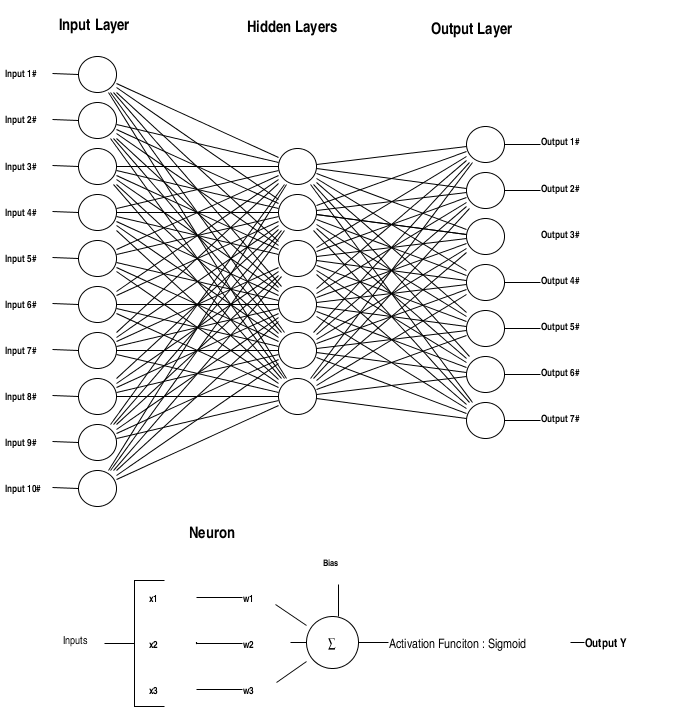
\includegraphics[width=11cm]{images/schemeit-project.png}
\caption{Schematic }
\label{schematic}
\end{center}
\end{figure}
\FloatBarrier


           \section{Training} \label {chapter:training}

The neural network that is implemented has to be trained to the type of data it will be processing. To do this the data from targets.txt is divided into a training, validation and test set. By changing the parameters of the network and comparing error's in the validation layer, the \enquote{optimal} parameters can be found.

\subsection{Dividing the data}
The data (7854 features with 10 inputs) is divided into 7 folds of 7854/7=1122 input lines each. 5 of these folds will be used for training and the other two for the test and validation set respectively. The purpose of the test fold is to observe the error percentage when the network is untrained  and thus uses random weight between -0.5 and -0.5. The training folds are used to train the network thus updating the weights of the network. After the network is trained the network processes the validation fold. For the validation fold the error percentage and sum of squared error's is calculated. Now the results from the test set and validation set can be compared and give insight in how well the network trained itself with the given parameters. 

\subsection{Evaluating the performace}
To evaluate the performance of different neural networks, lots of different neural networks with all different parameters will follow the same procedure mentioned above. The error percentage, sum of squared errors and the parameters are then stored for each network in a single txt file. 

The following parameters were changed for each network and checked for their influence:
\begin{itemize}
\item The learning rate $\alpha$
\item The amount of hidden layers
\item The amount of neurons per hidden layer
\item The amount of epochs of training
\end{itemize}

At the end, the parameters of the neural network which scored best,will be used for processing the unknown.txt inputs. 

 \subsection{The amount of training epochs}
 Because the neural network is implemented in Java code, the training epochs run quite fast therefore lets say thousand epochs, 1 hidden layer with 100 neurons will only take about ten minutes of training although it seems that after 30-50 epochs the error rate is not really improving anymore. To be sure in deciding the best parameters for the neural network, 100 epochs were run for each individual network.
 
 \subsection{Impact of the initialization}
 The initialization where each weight gets a random value between -0.5 and 0.5 does seem to effect the performance to some extend. Networks with the same parameters can have different outcomes which is expected because where the final \enquote{solution} converges, depends on the initial weights. 
           \section{Optimization} \label {chapter:optimization}

\subsection{Performance of different networks}
As described in \cref{chapter:training} different networks with different parameters can be compared to obtain the best parameters. \cref{test_val_error} shows the influence of changing the number of hidden neurons.

\begin{figure}[!h]
\begin{center}
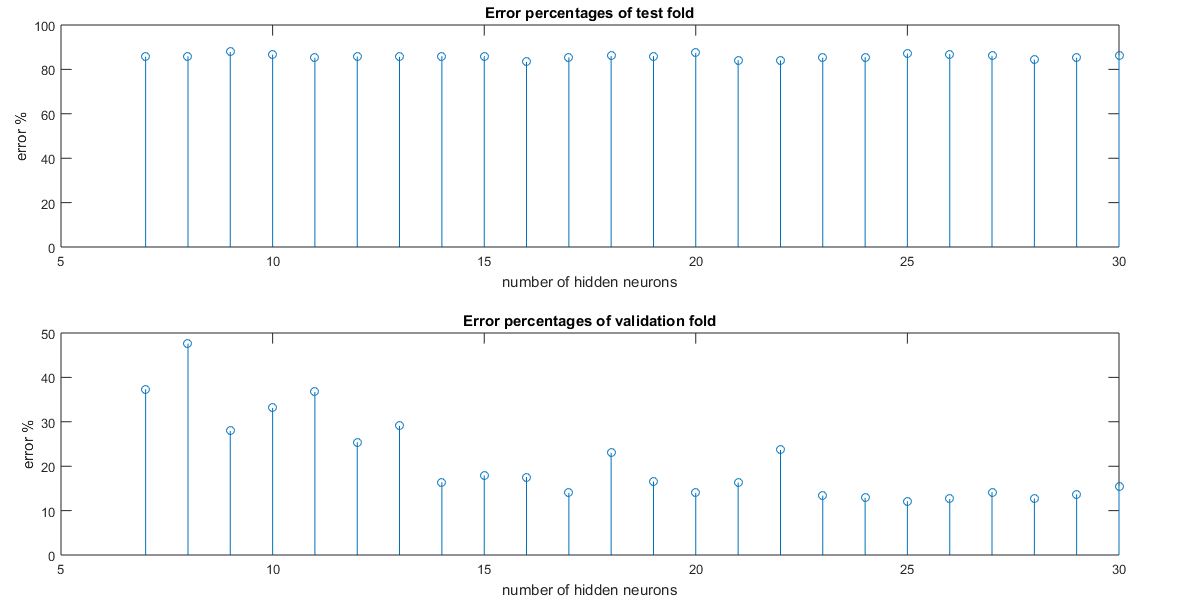
\includegraphics[width=16cm]{testresults/errorpercentages.png}
\caption{Error percentages of test and validation fold }
\label{test_val_error}
\end{center}
\end{figure}
           \section{Evaluation} \label {chapter:evaluation}

\subsection{Succes rate of the network}
Using the 1 hidden layer and 100 hidden neurons the error rate in the validation set was down to 2.67\% after 1000 epochs which corresponds to 30 errors of the (7854/7) targets in the validation set. In the test set the error percentage was 85.38\% with 958 errors. To show the dispersion of the errors a confusion plot was made from the outputs and targets using Matlab. The confusion matrix is show in \cref{confusion_matrix} and a plot of the values is show in \cref{confusion_plot}. 


\begin{figure}[!h]
\begin{center}
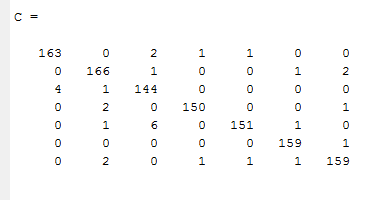
\includegraphics[width=8cm]{testresults/confusionmatrix.png}
\caption{Confusion matrix}
\label{confusion_matrix}
\end{center}
\end{figure}
\FloatBarrier

\begin{figure}[!h]
\begin{center}
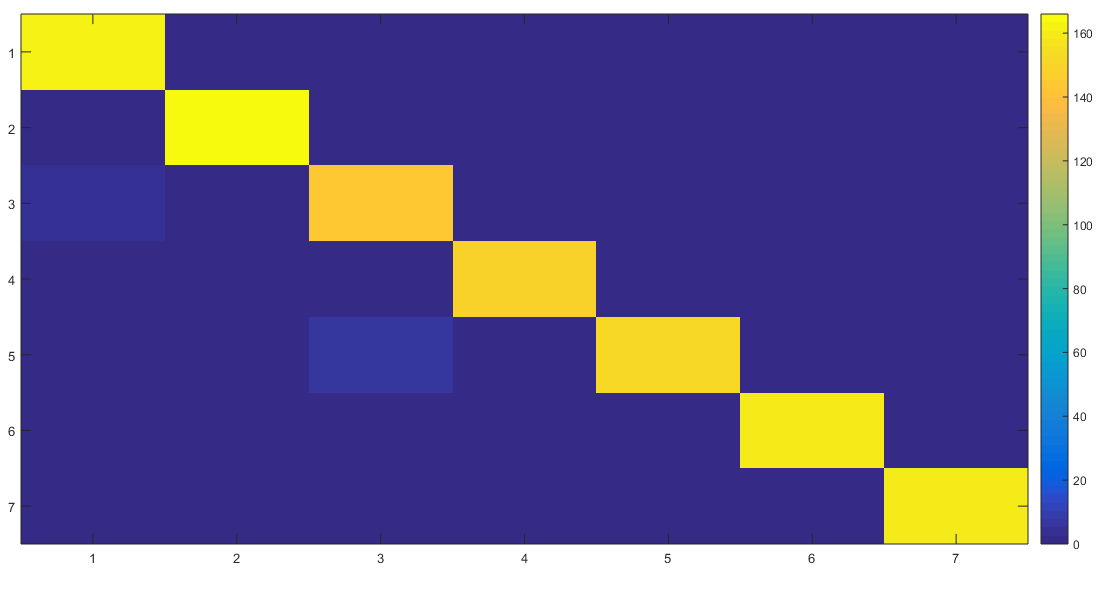
\includegraphics[width=6cm]{testresults/confusionplot.png}
\caption{Confusion plot}
\label{confusion_plot}
\end{center}
\end{figure}
\FloatBarrier

From the matrix and plot it can be concluded that the trained network works quite well on the validation set. The few errors that exist are somewhat evenly distributed over the whole set. Output number 3 has the highest error rate of 5.88\% with 9 error values from the 144+9=153 values.


  	\clearpage
%%%%%%%%%%%%%%%%%%%%%%%%%%%%%%%%%%%%%%%%%%%%%%%%%%%%%%%%%%%%%%%%%%%%%%
%							Bibliography
%%%%%%%%%%%%%%%%%%%%%%%%%%%%%%%%%%%%%%%%%%%%%%%%%%%%%%%%%%%%%%%%%%%%%%

    \bibliographystyle{plain}
	% bibliography

\begin{thebibliography}{99}










%EXAMPLES':
%	\bibitem{gs_book}	Rabaey J.M., Chandrakasan A., Nikoli\'{c} B., \emph{Digital Integrated Circuits: A Design Perspective, Second Edition}, Prentice Hall, New Jersey, 2003.
	
%	\bibitem{handleiding} N.P. van der Meijs \emph{Manual: EE2C11-courselab-1}, TU Delft, The Netherlands.
%	\bibitem{slides} N.P. van der Meijs \emph{Presentation slides Integrated Circuits}, Online: http://ens.ewi.tudelft.nl/~nick/courses/gs/slides.html.
	
%		\bibitem{software_matlab} Computer program \emph{MATLAB Version 8 R2012b}, (The Mathworks, 2012)	
%		\bibitem{software_pspice} Computer program \emph{PSPICE Version 9.1}, (Cadence Design Systems, 2000)
		
%	\bibitem{vhdl_book}	P. J. Ashenden, \emph{The student's guide to VHDL, Second Edition}, Morgan Kaufmann Publishers, Inc, San Francisco, 2008
%	\bibitem{datasheet_regulator} \emph{Datasheet LM1086}, National Semiconductor, Online: http://www.national.com/mpf/LM/LM1086.html
%	\bibitem{c_prac_handleiding} B. Jacobs, X. van Rijnsoever, A.J. van Genderen, \emph{Practicum Handleiding Programmeren in C}, TU Delft, The Netherlands
%	\bibitem{dijkstra} \emph{Dijkstra's kortste pad algoritme} Online: http://nl.wikipedia.org/wiki/Kortstepadalgoritme
%	\bibitem{lee_algo} \emph{Lee algoritme} Online: http://en.wikipedia.org/wiki/Lee\_algorithm
%	\bibitem{pong_chu}	Pong P. Chu, \emph{FPGA Prototyping by VHDL Examples}, 2008, John Wiley.
%	\bibitem{sio_win32}	R. Bayer, \emph{Windows Serial Port Programming}, 2008, Online: http://www.robbayer.com/files/serial-win.pdf
%	\bibitem{serial_comm} \emph{Serial Communications in Win32}, Microsoft , Online: http://msdn.microsoft.com/en-us/library/ms810467.aspx
%	\bibitem{xctu_manual}	DIGI, \emph{X-CTU User's Guide}, See: Blackboard EE1810->Resources
%	\bibitem{xbee_manual}	DIGI, \emph{XBee/XBee-PRO Manual v1}, See: Blackboard EE1810->Resources
%	\bibitem{datasheet_regulator} \emph{Datasheet LM1086}, National Semiconductor, Online: http://www.national.com/mpf/LM/LM1086.html
%	\bibitem{irwin_book}	 	J. David Irwin, R. Mark Nelms, \emph{Basic engineering circuit analysis}, Wiley, 2008.
%	\bibitem{datasheet_LF356} \emph{Datasheet LF155/LF156/LF256/LF257/LF355/LF356/LF357 JFET Input Operational Amplifiers}, National Semiconductor, Online: http://www.national.com/ds/LF/LF155.pdf.
%	\bibitem{datasheet_LM741} \emph{Datasheet LM741 Operation Amplifier}, National Semiconductor, Online: http://www.national.com/ds/LM/LM741.pdf.
\end{thebibliography}

	\clearpage

%%%%%%%%%%%%%%%%%%%%%%%%%%%%%%%%%%%%%%%%%%%%%%%%%%%%%%%%%%%%%%%%%%%%%%
%								Appendix
%%%%%%%%%%%%%%%%%%%%%%%%%%%%%%%%%%%%%%%%%%%%%%%%%%%%%%%%%%%%%%%%%%%%%%
	\clearpage
    \appendix
		%EXAMPLE:
		%\input{appendix_matlabcode}
        
%%%%%%%%%%%%%%%%%%%%%%%%%%%%%%%%%%%%%%%%%%%%%%%%%%%%%%%%%%%%%%%%%%%%%%
\end{document}